\myslide{Outline}
{
  \begin{itemgroup}{Übersicht}
    \item Ausdrücke und Typen können in ihrer Baumansicht betrachtet werden
    \item Schwierige Ausdrucke können so besser verstanden werden
    \item Name der Ausdücke und Typen wird dargestellt
    \item Menge der Ausdrücke und Typen wird dargestellt
    \item Der Index wird ebenfalls eingeblendet
    \item Bindungen von Identifiern können betrachtet werden
    \item Die Outline muss bei neuen Ausdrücken nicht angepasst werden,
          sondern übernimmt diese automatisch
  \end{itemgroup}
}

\myslide{Outline}
{
  \begin{itemgroup}{Einstellungen}
    \item \glqq Hervorheben\grqq: Selektierte Knoten werden in höheren Knoten markiert
    \item \glqq Gebundene\grqq: Gebundene Identifier werden markiert
    \item \glqq Freie\grqq: Frei vorkommende Identifier werden markiert
    \item \glqq Ersetzen\grqq: Selektierte Knoten werden durch \glqq ...\grqq\ ersetzt
    \item \glqq Source Code\grqq: Der zu dem selektierten Knoten passende Source Code
                                  wird im Editor hervorgehoben
    \item \glqq Auto Update\grqq: Die Outline wird bei Änderungen automatisch aktualisiert
  \end{itemgroup}
}

\myslide{Outline}
{
  \begin{center}
    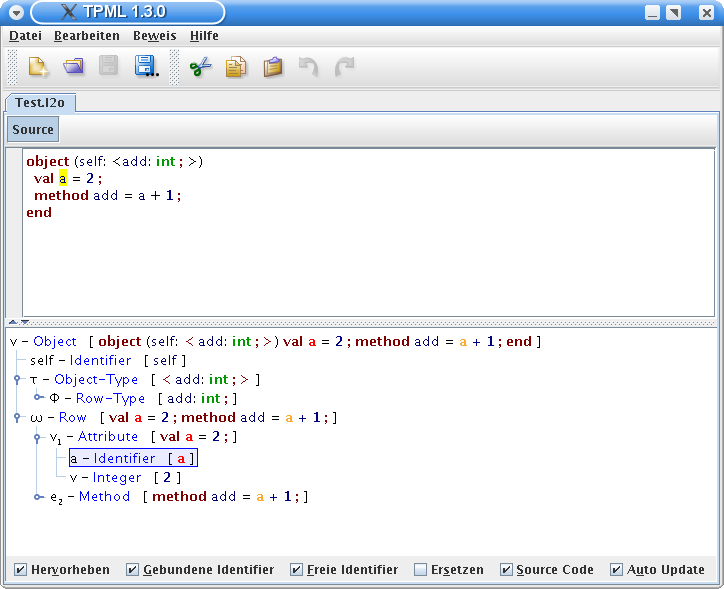
\includegraphics[height=15cm]{images/outline.png}
  \end{center}
}